% Section: Category Theory: The Ultimate Abstraction

The answer came from algebra, not logic---but it turned out to be exactly what logic needed.

In the 1940s, Samuel Eilenberg and Saunders Mac Lane, studying algebraic topology, noticed something curious: many proofs weren't really about specific objects (groups, spaces, modules). They were about \textbf{relationships between objects}---homomorphisms, continuous maps, natural transformations.

The objects were interchangeable; the arrows were what mattered.

They invented \textbf{category theory} to capture this.

\subsection{Informal Picture}

Think of a category as a world of objects connected by arrows:

\begin{itemize}
    \item \textbf{Objects} are the ``things''---sets, groups, spaces, whatever. We don't care what they're made of internally.
    \item \textbf{Morphisms} (arrows) are the ``relationships'' between objects. An arrow $f: A \to B$ goes from $A$ to $B$.
    \item \textbf{Composition}: If you can go from $A$ to $B$, and from $B$ to $C$, you can go from $A$ to $C$. Arrows chain together.
    \item \textbf{Identity}: Every object has a ``do nothing'' arrow to itself.
\end{itemize}

\begin{center}
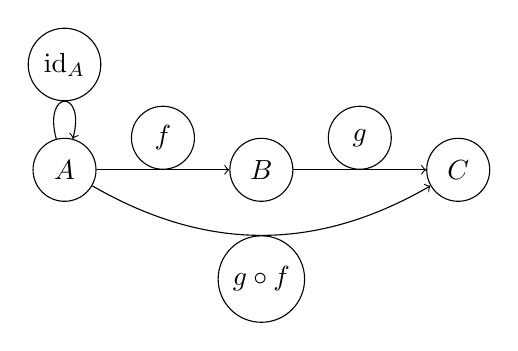
\begin{tikzpicture}[node distance=2.5cm, every node/.style={circle, draw, minimum size=0.8cm}]
    \node (A) {$A$};
    \node (B) [right of=A] {$B$};
    \node (C) [right of=B] {$C$};
    \draw[->] (A) to node[above] {$f$} (B);
    \draw[->] (B) to node[above] {$g$} (C);
    \draw[->, bend right=30] (A) to node[below] {$g \circ f$} (C);
    \draw[->] (A) to [loop above] node {$\mathrm{id}_A$} (A);
\end{tikzpicture}
\end{center}

\subsection{Formal Definition}

\begin{definition}[Category]
A \textbf{category} $\mathcal{C}$ consists of:
\begin{itemize}
    \item A collection $\mathrm{Ob}(\mathcal{C})$ of \textbf{objects}
    \item For each pair of objects $A, B$, a collection $\mathrm{Hom}(A, B)$ of \textbf{morphisms} from $A$ to $B$
    \item For each object $A$, an \textbf{identity morphism} $\mathrm{id}_A \in \mathrm{Hom}(A, A)$
    \item For each triple $A, B, C$, a \textbf{composition operation}:
    \[ \circ : \mathrm{Hom}(B, C) \times \mathrm{Hom}(A, B) \to \mathrm{Hom}(A, C) \]
\end{itemize}
satisfying:
\begin{enumerate}
    \item \textbf{Associativity:} $(h \circ g) \circ f = h \circ (g \circ f)$

    \textit{``It doesn't matter how you group compositions---the result is the same.''}

    \item \textbf{Identity laws:} $f \circ \mathrm{id}_A = f$ and $\mathrm{id}_B \circ f = f$ for any $f: A \to B$

    \textit{``Composing with identity does nothing.''}
\end{enumerate}
\end{definition}

\subsection{Why These Axioms?}

The axioms capture the minimal requirements for ``things and transformations between them'':

\begin{itemize}
    \item \textbf{Associativity} says composition is well-behaved. If you transform $A \to B \to C \to D$, you get the same result whether you first compose $A \to B \to C$ and then go to $D$, or first compose $B \to C \to D$ and apply $A$ to that. No ambiguity.

    \item \textbf{Identity} says every object has a trivial ``self-transformation.'' This is like the number $0$ for addition or $1$ for multiplication---it's the ``do nothing'' operation.
\end{itemize}

\begin{example}[Some categories]\leavevmode
\begin{itemize}
    \item $\mathbf{Set}$: objects are sets, morphisms are functions, composition is function composition, identity is the identity function $x \mapsto x$.

    \item $\mathbf{Grp}$: objects are groups, morphisms are group homomorphisms (functions that preserve the group operation), composition and identity as in $\mathbf{Set}$.

    \item $\mathbf{Top}$: objects are topological spaces, morphisms are continuous maps.

    \item $\mathbf{Pos}$: objects are partially ordered sets, morphisms are monotone functions ($x \leq y \Rightarrow f(x) \leq f(y)$).

    \item $\mathbf{Vect}_k$: objects are vector spaces over field $k$, morphisms are linear maps.
\end{itemize}
\end{example}

\begin{intuition}
Notice the pattern: in each case, morphisms are ``structure-respecting maps.'' Functions respect set structure (elements map to elements). Homomorphisms respect group structure ($f(ab) = f(a)f(b)$). Continuous maps respect topological structure (preimages of open sets are open).

A category isolates this pattern: objects have some structure, morphisms respect it. We can then study properties that depend only on this pattern, not on the specific structures involved.
\end{intuition}

\begin{keyinsight}
Category theory is the \textbf{mathematics of mathematics}. It studies structure and invariance in full generality.

This is exactly what logic needed: a language where \emph{transformations} and \emph{what they preserve} are first-class concepts.
\end{keyinsight}
